\documentclass[border=3pt]{standalone}
% Shared preamble for standalone figures (same fonts/colours as the paper).
\usepackage[T1]{fontenc}
\usepackage{lmodern}
\usepackage{amsmath,amssymb}
\usepackage[dvipsnames,svgnames]{xcolor}
\usepackage{tikz}
\usetikzlibrary{arrows.meta,positioning,calc,shapes.geometric,decorations.pathreplacing,shadings}
\usepackage{pgfplots}
\pgfplotsset{compat=1.18}
\usepgfplotslibrary{fillbetween}
\definecolor{pgrey}{HTML}{EEEEEE}
\definecolor{ppink}{HTML}{F8D7DA}
\definecolor{ppeach}{HTML}{FDE5C8}
\definecolor{porange}{HTML}{FBC78D}
\definecolor{pgreen}{HTML}{D4F7D4}
\definecolor{ppurple}{HTML}{EFE3F7}
\definecolor{pblue}{HTML}{DCE8F7}
\definecolor{dgreen}{HTML}{2E8B2E}
\definecolor{dpink}{HTML}{C2185B}
\definecolor{dorange}{HTML}{E07B00}
\definecolor{dblue}{HTML}{1F4E9E}
\definecolor{dpurple}{HTML}{7B3FA0}
\definecolor{gold}{HTML}{E0A800}
\tikzset{
  blk/.style={draw=black!70,rounded corners=2pt,minimum height=0.8cm,minimum width=1.9cm,
              align=center,font=\sffamily\footnotesize,inner sep=3pt},
  arr/.style={-{Stealth[length=2.2mm]},thick,black!75},
  darr/.style={-{Stealth[length=2mm]},dashed,thick},
  lbl/.style={font=\itshape\scriptsize},
}

\begin{document}
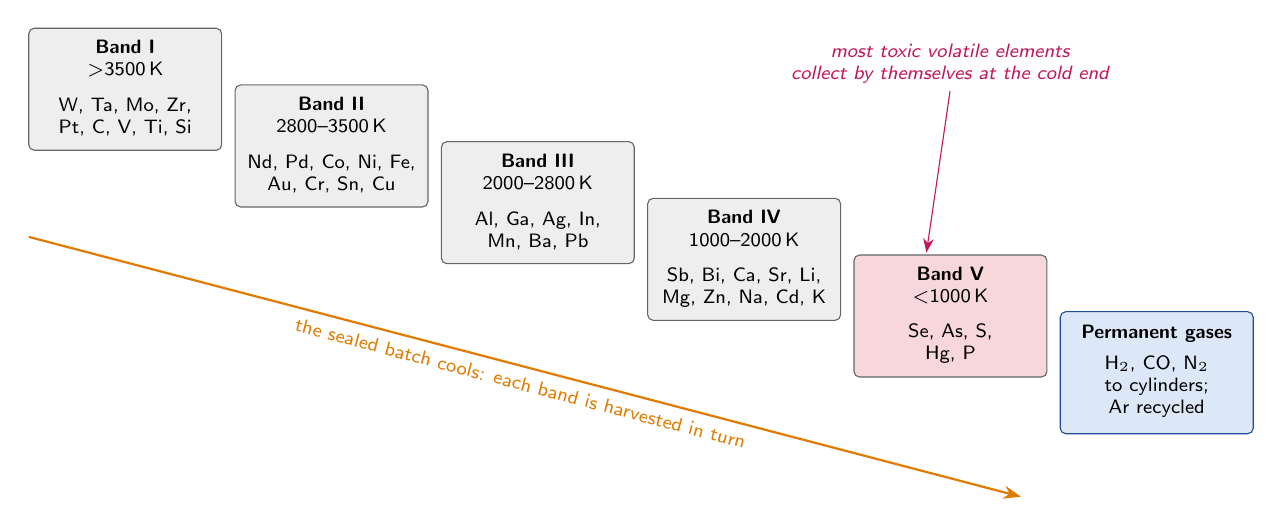
\begin{tikzpicture}[x=1cm,y=1cm]
\foreach \i/\name/\range/\els/\fill in {
  0/Band I/{$>$3500\,K}/{W, Ta, Mo, Zr,\\Pt, C, V, Ti, Si}/pgrey,
  1/Band II/{2800--3500\,K}/{Nd, Pd, Co, Ni, Fe,\\Au, Cr, Sn, Cu}/pgrey,
  2/Band III/{2000--2800\,K}/{Al, Ga, Ag, In,\\Mn, Ba, Pb}/pgrey,
  3/Band IV/{1000--2000\,K}/{Sb, Bi, Ca, Sr, Li,\\Mg, Zn, Na, Cd, K}/pgrey,
  4/Band V/{$<$1000\,K}/{Se, As, S,\\Hg, P}/ppink}{
  \pgfmathsetmacro\x{\i*2.62}\pgfmathsetmacro\y{-\i*0.72}
  \draw[fill=\fill,draw=black!60,rounded corners=2pt] (\x,\y) rectangle (\x+2.45,\y+1.55);
  \node[font=\sffamily\scriptsize,anchor=north,align=center] at (\x+1.225,\y+1.52) {\textbf{\name}\\\range};
  \node[font=\sffamily\scriptsize,align=center] at (\x+1.225,\y+0.42) {\els};}
\draw[fill=pblue,draw=dblue,rounded corners=2pt] (13.1,-3.6) rectangle (15.55,-2.05);
\node[font=\sffamily\scriptsize\bfseries,anchor=north] at (14.325,-2.1) {Permanent gases};
\node[font=\sffamily\scriptsize,align=center] at (14.325,-3.0) {H$_2$, CO, N$_2$\\to cylinders;\\Ar recycled};
\draw[-{Stealth[length=2.2mm]},thick,dorange] (0,-1.1) -- node[below,font=\sffamily\scriptsize,sloped]{the sealed batch cools: each band is harvested in turn} (12.6,-4.4);
\node[font=\sffamily\scriptsize\itshape,text=dpink,align=center] at (11.7,1.1) {most toxic volatile elements\\collect by themselves at the cold end};
\draw[dpink,-{Stealth[length=1.8mm]}] (11.7,0.75) -- (11.4,-1.3);
\end{tikzpicture}
\end{document}
